\subsection{Python}

% Introduction {{{
\begin{figure}[H]
  \centering
  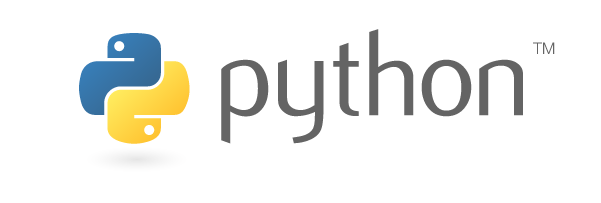
\includegraphics[width=\linewidth/2]{%
    diagrams/python_logo.png}
  \caption{Python Logo}
\end{figure}

At the point when computers came to presence in their
initial years, there was the need for them to be modified.

Computer scientists came with a 0 and 1 programming
language as the optimum solution at that time, yet it was
extremely troublesome and tedious. This trouble caused
great advancements in programming and prompted the
processes of making high level languages that we know and
hear about nowadays.

Python is a general-purpose high-level programming
language\cite{amjad1} whose design philosophy
emphasizes code readability.\cite{amjad2}

Python aims to combine "remarkable power with very clear
syntax"\cite{amjad3} and its standard library is large and
comprehensive. Its use of indentation for block delimiters
is unusual among popular programming languages.

Python can be considered as a multi-paradigm programming
language. Rather than forcing programmers to adopt a
particular style of programming, it permits several styles:
object-oriented programming and structured programming also
are fully supported. Many other paradigms are supported
using extensions, such as pyDBC\cite{amjad4} and Contracts
for Python\cite{amjad5} which allow Design by Contract.

Python uses dynamic typing and a combination of reference
counting and a cycle-detecting garbage collector for memory
management. An important feature of Python is dynamic name
resolution (late binding), which binds method and variable
names during program execution.

Rather than requiring all desired functionality to be built
into the language's core, Python was designed to be highly
extensible. New built-in modules can be easily written in
C, C++. Python can also be used as an extension language
for existing modules and applications that need a
programmable interface. This design of a small core
language with a large standard library andan easily
extensible interpreter was intended by Van Rossum from the
very start because of his frustrations with ABC (which
espoused the opposite mindset).\cite{amjad6}

Like other dynamic languages, Python is often used as a
scripting language, but is also used in a wide range of
non-scripting contexts. Using third-party tools, such as
Py2exe or Pyinstaller\cite{amjad7},
Python code can be packaged into standalone executable
programs. Python interpreters are available for many
operating systems.
% }}}

% History {{{
\subsubsection{History}

Python was conceived in the late 1980s\cite{amjad8} and its
implementation was getting started in December 1989
\cite{amjad9} by Guido van Rossum at CWI in the Netherlands
as a successor to the ABC programming language (itself
inspired by SETL)\cite{amjad10} capable of exception
handling and interfacing with the Amoeba operating system.
\cite{amjad11}

Van Rossum is Python's principal author, and his continuing
central role in deciding the direction of Python is
reflected in the title given to him by the Python
community, Benevolent Dictator for Life (BDFL).

Python 2.0 was released on 16 October 2000, with many major
new features including a full garbage collector and support
for Unicode. However, the most important change was to the
development process itself, with a shift to a more
transparent and community-backed process.

Python 3.0, a major, backwards-incompatible release, was
released on 3 rd of December 2008\cite{amjad12}
after a long period of testing. Many of its major features
have been back-ported to the backwards-compatible Python
2.7.\cite{amjad13}
% }}}

% What is Python ? {{{
\subsubsection{What is Python?}

Python is a high-level programming language designed to be
easy to read and simple to implement. It is open source,
which means it is free to use, even for commercial
applications.

Python can run on Mac, Windows, and UNIX operating systems
and has also been ported to Java and .NET virtual machines.
\cite{amjad14}

Python is considered a scripting language, like Ruby or
Perl and is often used for creating Web applications and
dynamic Web content. It is also supported by a number of 2D
and 3D imaging programs, enabling users to create custom
plug-ins and extensions with Python. Examples of
applications that support a Python API include GIMP,
Blender, and Autodesk Maya.\cite{amjad14}

Python supports the use of modules and packages, which
means that programs can be designed in a modular style and
code can be reused across a variety of projects. Once the
user develops a module or package she/he needs, it can be
scaled for use in other projects, and it's easy to import
or export these modules.\cite{amjad15}

Scripts written in Python (.py files) can be parsed and run
immediately. They can also be saved as a compiled programs
(.pyc files), which are often used as programming modules
that can be referenced by other Python programs.
\cite{amjad14}

That being said, it can be considered that python has a lot
of distinguishing properties and features as being portable
since, it can be used on a lot of operating systems. In
addition there are some other properties such:

\begin{enumerate}

  \item Python supports other technologies:

        It can support COM, .Net, etc. objects. Also, some
        alternatives and complements were created for
        Python that make it easier to work with these
        objects in an integrated mode.

  \item Presence of Third Party Modules:

        The Python Package Index (PyPI) contains numerous
        third-party modules that make Python capable of
        interacting with most of the other languages and
        platforms.\cite{amjad16}

  \item Python is open source:

        Even though all rights of this program are reserved
        for the Python institute, but it is open source and
        there is no limitation in using, changing and
        distributing.\cite{amjad17}

  \item Learning Ease and Support Available:

        Python offers excellent readability and uncluttered
        simple-to-learn syntax which helps beginners to
        utilize this programming language. The code style
        guidelines, PEP 8, provide a set of rules to
        facilitate the formatting of code. Additionally,
        the wide base of users and active developers has
        resulted in a rich internet resource bank to
        encourage development and the continued adoption of
        the language.\cite{amjad16}

  \item Productivity and Speed:

        Python has clean object-oriented design, provides
        enhanced process control capabilities, and
        possesses strong integration and text processing
        capabilities and its own unit testing framework,
        all of which contribute to the increase in its
        speed and productivity. Python is considered a
        viable option for building complex multi-protocol
        network applications.\cite{amjad16}

\end{enumerate}
% }}}

% Features and philosophy {{{
\subsubsection{Features and philosophy}

Python uses dynamic typing and a combination of reference
counting and a cycle-detecting garbage collector for memory
management. An important feature of Python is dynamic name
resolution (late binding), which binds method and variable
names during program execution.\cite{amjad18}

The design of Python offers only limited support for
functional programming in the Lisp tradition. The language
has map, reduce and filter functions, comprehensions for
lists, dictionaries, and sets, as well as generator
expressions.\cite{amjad19} The standard library has two
modules (itertools and functools) that implement functional
tools borrowed from Haskell and Standard ML.\cite{amjad20}

An important goal of the Python developers is making Python
fun to use. This is reflected in the origin of the name
which comes from Monty Python, and in an occasionally
playful approach to tutorials and reference materials, for
example using spam and eggs instead of the standard foo
and bar.\cite{amjad21}

Python has a large standard library, commonly cited as one
of Python's greatest strengths, providing tools suited for
many tasks. This is deliberate and has been described as a
"batteries included" Python philosophy. For Internet-facing
applications, a large number of standard formats and
protocols (such as MIME and HTTP) are supported. Modules
for creating graphical user interfaces, connecting to
relational databases, pseudorandom number generators,
arithmetic with arbitrary precision decimals, manipulating
regular expressions, and doing unit testing are also
included.\cite{amjad21}

Some parts of the standard library are covered by
specifications (for example, the WSGI implementation
wsgiref follows PEP 333), but the majority of the modules
are not. They are specified by their code, internal
documentation, and test suite (if supplied). However,
because most of the standard library is cross-platform
Python code, there are only a few modules that must be
altered or completely rewritten by alternative
implementations.\cite{amjad21}

The standard library is not essential to run Python or
embed Python within an application. Blender 2.49 for
instance omits most of the standard library.

\begin{figure}[H]
  \centering
  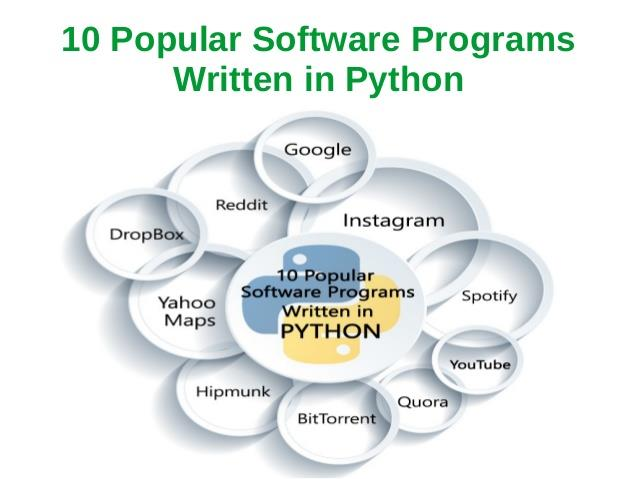
\includegraphics[width=\linewidth/2]{%
    diagrams/programs_written_in_python.png}
  \caption{Popular software written in Python}
\end{figure}
% }}}

% Why we took Python for our project {{{
\subsubsection{Why we took Python for our project}

Python is a well-designed language that can be used for
real world programming. Some of its strengths were very
appealing to us when we thought about which language to
use.

The most obvious strength and the reason we decided to use
Python are the libraries,
frameworks and APIs for machine learning written for/in
Python (especially Tensorflow and Keras, which we used, but
including far more well designed and beloved tools like
PyTorch, Theano, matplotlib, etc).

Here are some other strengths of Python we really
appreciated during development:

\begin{itemize}

  \item System programming:

        Internal interfaces of python that are created for
        working with services of operating system cause
        Python to be a suitable language for system
        programming.

        These interfaces provide some functions such as:
        files and directories operations, parallel
        processing, etc. the standard library of Python can
        support the different types of platforms and
        operating systems. It contains some tools for
        working with system resources such as:
        environmental variables, files, sockets, pipes,
        processes, multiple treats, command line, standard
        stream interfaces, shell programming, etc.
        \cite{amjad21}


  \item Network and internet programming:

        Various modules are embedded in Python standard
        library that provide many tools for network
        programmers, such as: client-server connection,
        socket programming, FTP, Telnet, email functions,
        RPC, SOAP, etc.

        Also, some third-party tools like mod-Python allow
        web servers like apache to run Python scripts.
        Furthermore, some popular programs such as: Django,
        Turbo gears, Pylon, Zope and Web Ware support
        Python scripts.\cite{amjad21}

  \item Numerical programming:

        Python with the NumPy library for Linear Algebra
        computations (used in Tensorflow) can be a powerful
        alternative for FORTRAN and C++, because it
        provides powerful tools for working with
        mathematical libraries, by using simple Python
        code. Also, there are many third-party tools on
        the internet for numerical computations.

\end{itemize}
% }}}
